
\medskip

\emph{Cet exercice est composé de trois situations qui n’ont pas de lien entre elles.}

\medskip

\begin{minipage}[t]{0.48\linewidth}
	\textbf{Situation 1 :}

	\medskip

On considère le programme de calcul ci-contre :
\end{minipage}\hfill
\begin{minipage}[t]{0.48\linewidth}
	\begin{center}
%		\begin{tikzpicture}[]
%			\node (A) at (0,0) [draw, align = center,text width = 3.2cm] {nombre de départ};
%			\node [shift={(0,-1)}, below, draw, align=center, text width=7cm] at (A.south) (B) {
%				Soustraire 7.\linebreak
%				Multiplier par 5.\linebreak
%				Soustraire le double du nombre de départ.};
%			\node [shift={(0,-1)},draw, below, align = center,text width = 3.5 cm] at (B.south) (B)(C)  {Résultat};
%			\draw[->, line width=2mm, > = stealth] (A.south)--(B.north);
%			\draw[->, line width=2mm, > = stealth] (B.south)--(C.north);
%		\end{tikzpicture}
		\psset{unit=1cm}
		\begin{pspicture}(-3.7,-0.5)(3.7,-5)
		%\psgrid
		\rput(0,-0.8){Nombre de départ}
		\psframe(-1.7,-0.5)(1.7,-1)
		\psline[linewidth=4.5pt]{->}(0,-1)(0,-1.8)
		\rput(0,-2.1){Soustraire 7}
		\rput(0,-2.5){Multiplier par 5.}
		\rput(0,-2.9){Soustraire le double du nombre de départ}
		\psline[linewidth=4.5pt]{->}(0,-3.2)(0,-4.1)
		\psframe(-3.6,-1.8)(3.6,-3.2)
		\rput(0,-4.45){Résultat}
		\psframe(-1.6,-4.2)(1.6,-4.7)
		\end{pspicture}
	\end{center}
\end{minipage}



\begin{enumerate}
	\item Montrer que si le nombre de départ est 10, le résultat obtenu est $-5$.

	\item On note $x$ le nombre de départ auquel on applique ce programme de calcul.

	Parmi les expressions suivantes, quelle est celle qui correspond au résultat du programme de calcul ? \emph{Aucune justification n’est attendue pour cette question}.

%	\begin{tblr}{colspec={@{}l X[$] l X[$]}}
%		Expression A: & x-7 \times 5-2x   &Expression B: & 5(x-7)- 2x\\
%		Expression C: & 5(x-7)-x^2 &Expression D: & 5x -7- 2x	\\
%	\end{tblr}
\begin{tabularx}{\linewidth}{*{2}{X}}
Expression A : $x - 7 \times  5 - 2x$& Expression C : $5(x - 7) - 2x$\\
Expression B : $5(x - 7) - x^2$& Expression D : $5x - 7 - 2x$\\
\end{tabularx}
\end{enumerate}

\medskip

\begin{minipage}[t]{0.48\linewidth}
	\textbf{Situation 2 :}

Dans le repère ci-contre, la droite (d) représente une fonction linéaire $f$.

Le point A appartient a la droite (d).

\begin{enumerate}
	\item À l’aide du graphique, déterminer l’image de $- 2$ par la fonction $f$.

	\item Déterminer une expression de $f(x)$ en fonction de $x$.
\end{enumerate}
\end{minipage}
\hfill
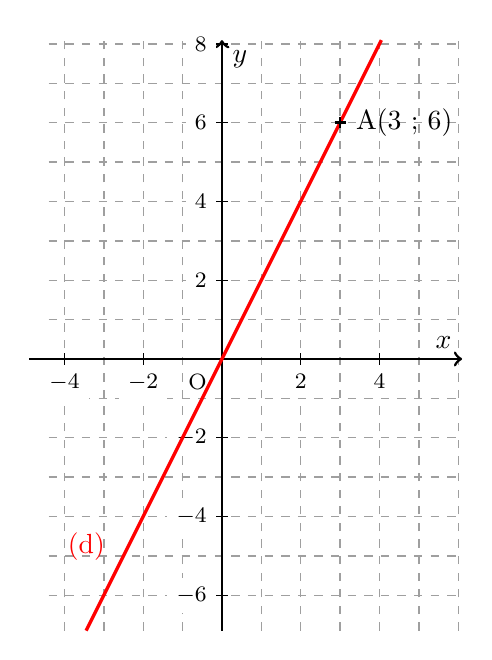
\begin{tikzpicture}[baseline={(Y.base)}, x= 5mm, y = 5mm]
	\draw [color = gray!75, line width = 0.5pt, dashed, xstep=1, ystep = 1] (-4.4,-6.9) grid (6.1,8.1);
	\draw[line width = 1pt, ->] (-4.9,0) -- (6.1,0) node[above left] {$x$};
	\foreach \x in {-4,-2,2,4}
	\draw[shift={(\x,0)},color=black] (0pt,2pt) -- (0pt,-2pt) node[below, fill = white] {\footnotesize $\np{\x}$};
	\draw[line width = 1pt, ->] (0,-6.9) -- (0,8.1) node[below right] (Y) {$y$};
	\foreach \y in {-6,-4,-2,2,4,6,8}
	\draw[shift={(0,\y)},color=black] (2pt,0pt) -- (-2pt,0pt) node[left, fill = white] {\footnotesize $\np{\y}$};
	\draw[color=black] (-2pt,-2pt) node[below left] {{\footnotesize  O}};
	\draw[line width=1.2pt,color=red] (-3.45,-6.9)--(4.05,8.1) node[pos=0.1, above left]{(d)};
	\draw[line width=1pt,shift={(3,6)}] (0,2pt)--(0,-2pt) (-2pt,0)--(2pt,0) node[right] {A(3 ; 6)};
\end{tikzpicture}

\medskip
\textbf{Situation 3}

%\begin{tblr} {@{}X[2]X[2,c]X}
%	Le dessin ci-contre représente une pyramide de sommet G et dont la base CDEF est un rectangle.
%
%Le volume de cette pyramide est-il supérieur a 20 L ?&
%\begin{tikzpicture}[line width=1pt, baseline=(G.base), ]
%	\draw (-1.1,0.7) node[above left] {E} -- (0,0) node[below] {D} -- (3.3,0.4) node[right]{C} -- (1.1,3.7) node[above] (G){G} -- cycle
%	(1.1,3.7)--(0,0);
%	\draw[dashed] (0,0) -- (2.2,1.1) node[above right] {F} -- (1.1,3.7)
%	(3.3,0.4) -- (-1.1,0.7) -- (2.2,1.1) -- cycle
%	(1.1,3.7)--(1.1,0.55) node[below]{H};
%	\draw[line width=0.7pt] (1.1,0.55)--(0.9,0.45)--(0.9,0.8)--(1.1,0.9) -- cycle;
%	\draw[line width=0.7pt] (1.1,0.55)--(1.4,0.53) -- (1.4,0.88)--(1.1,0.9) -- cycle;
%\end{tikzpicture}&
%ED = 30 cm
%
%DC = 40 cm
%
%GH = 55 cm
%\end{tblr}

\begin{minipage}{0.48\linewidth}
Le dessin ci-contre représente une pyramide de sommet G et dont la base CDEF est un rectangle.

Le volume de cette pyramide est-il supérieur à 20 L ?
\end{minipage}\hfill
\begin{minipage}{0.48\linewidth}
\psset{unit=1cm}
\begin{pspicture}(6.6,4.5)
%\psgrid
\pspolygon(2.4,4)(0.3,1)(1.4,0.4)%GED
\psline(1.4,0.4)(4.5,0.7)(2.4,4)%DCG
\psline[linestyle=dashed](1.4,0.4)(3.4,1.3)(2.4,4)(2.4,1)%DFGH
\pspolygon[linestyle=dashed](0.3,1)(3.4,1.3)(4.5,0.7)%EFCE
\uput[r](4.5,0.7){\small C} \uput[dl](1.4,0.4){\small D} \uput[l](0.3,1){\small E} 
\uput[ur](3.4,1.3){\small F} \uput[u](2.4,4){\small G} \uput[d](2.4,1){\small H}
\uput[r](4.5,4){ED = 30 cm} \uput[r](4.5,3){DC = 40 cm}\uput[r](4.5,2){GH = 55 cm}
\psline(2.4,1)(2.6,0.96)(2.6,0.82)
\psline(2.4,1)(2.2,0.93)(2.2,0.83)
\end{pspicture}
\end{minipage}

\medskip

